\chapter{Evaluation}
In this chapter, we introduce the provided datasets we evaluate the models on.
We then set hypotheses about the assumed performances of the chosen models on
our datasets. Next, we describe our process of training. We briefly mention the
technologies we have used and how we have chosen our models' parameters.
Finally, we present our achieved results and discuss them.

\section{Datasets}
We are provided with three datasets by the company SANEZOO. Unfortunately, two
of the datasets cannot be published as they are protected under a
confidentiality agreement. However, we provide sufficient characteristics of the
datasets. We summarize the basic information of the datasets in Table
\ref{tab:datasets}. Detailed description is provided below the table.
\todo{Doplnit chybejici udaje.}

\begin{table}[h]
	\centering
	\begin{tabular}{|l|l|l|l|l|}
		\hline
		\bld{Type}       & \bld{Difficulty} & \bld{Size}             & \bld{Classes}          & \bld{Publishable} \\ \hline
		Candies          & Easy             & 150                    & 1                      & Yes               \\
		Metal parts      & Medium           & 5790                   & 7                      & No                \\
		Medical supplies & Hard             & \textit{bude doplneno} & \textit{bude doplneno} & No                \\ \hline
	\end{tabular}
	\caption{Datasets summary.}
	\label{tab:datasets}
\end{table}


\begin{figure}[H]

	\begin{subfigure}[c]{0.5\textwidth}
		\centering
		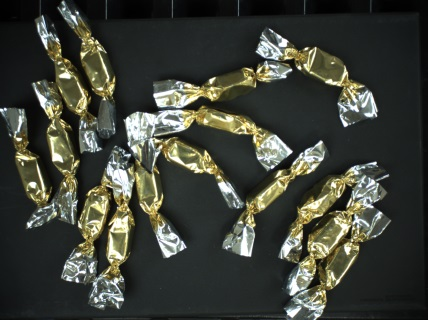
\includegraphics[width=0.9\linewidth]{Sources/Figures/sparse.jpg}
		\caption{Sparse example}

	\end{subfigure}
	\begin{subfigure}[c]{0.5\textwidth}
		\centering
		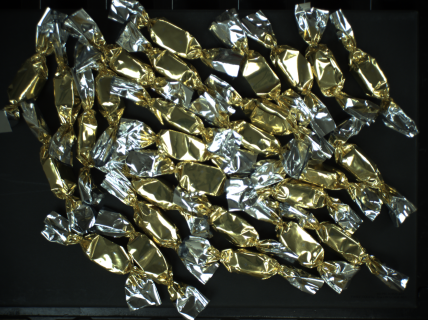
\includegraphics[width=0.9\linewidth]{Sources/Figures/dense.png}
		\caption{Dense example}

	\end{subfigure}

	\caption{Examples of candies dataset.}
	\label{fig:candies}
\end{figure}

\bld{Candies dataset.} Only the first dataset is publishable; thus, we provide a
visual example image in Figure \ref{fig:candies}. The images consist only of a
single class -- a golden candy. The density of objects (how densely they cover
the image) varies through the dataset (see Figure \ref{fig:candies}). Object
occlusions can occur in dense images; therefore, the dataset is not trivial.
However, compared to our other datasets, it is still a simpler dataset as it
strictly contains only a single class without foreign objects. Therefore, we
assign an easy difficulty to this dataset.


\bld{Metal parts dataset.} The second dataset consists of images with small
metal parts (such as shafts, rings, casings). See Figure \ref{fig:parts} for
rough illustration. The objects are placed in a plastic bin. There is always
only one class of objects on a single image. The images are taken from a
top-down perspective, similarly as in Figure \ref{fig:candies}. However, they
are taken from various angles. The density of objects also differ through the
dataset as in the first dataset (you can imagine a pile of metal parts).

\begin{figure}[ht]
	\centering
	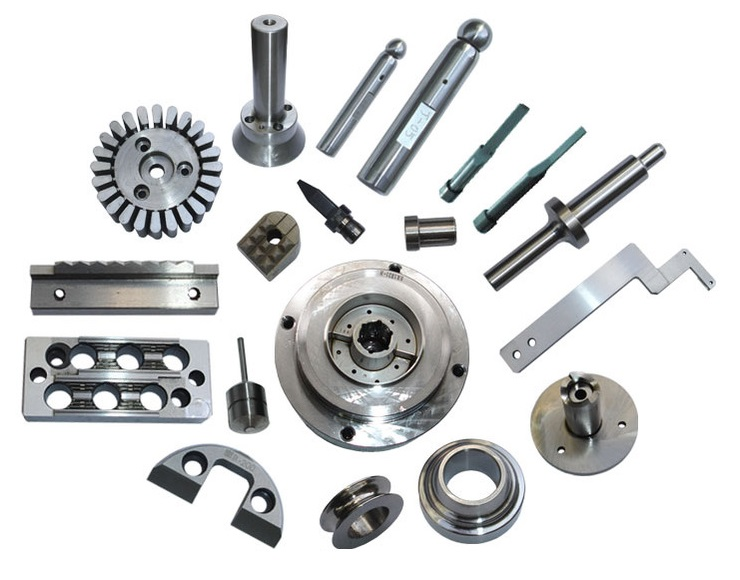
\includegraphics[height=0.35\linewidth]{Sources/Figures/metal_parts.jpg}
	\caption{An illustration of classes from metal parts dataset. Taken from
		\cite{parts}.}
	\label{fig:parts}
\end{figure}

\bld{Medical supplies dataset} The last set is made up of sequences of images
taken from an assembly line's top view. The images capture a manual assembly of
packages that are consisted of medical items (such as bandages, plastic cups, or
surgery tools). We assign a hard difficulty to this dataset because of the
non-static environment. To be more specific, the packages are in motion in some
images; therefore, the objects are slightly blurred. Moreover, occlusion of
objects occurs in the image very often since the operator does the packing
manually, and the objects are stacked on top of each other. Some objects are
tough to distinguish if they are next to each other (imagine a pile of cotton
balls). The images are taken from above the operator similarly as in the first
dataset.

\section{Hypotheses}
Let us recapitulate the models we evaluate:
\begin{itemize}
	\item Faster R-CNN with ResNet-50 backbone without FPN (Faster R-CNN),
	\item Cascade R-CNN with ResNet-50 backbone with FPN (Cascade R-CNN),
	\item RetinaNet with ResNet-50 backbone with FPN (RetinaNet R-50).
\end{itemize}
Additionally, we perform an experiment on RetinaNet with ResNet-101 and FPN
(see next). We set these hypotheses based on the results observed in the
models' original papers and the \bld{Detectron2's} benchmark.
\renewcommand{\theenumi}{\alph{enumi}}
\begin{enumerate}
	\item Faster R-CNN serves as a baseline and will perform the worst on every
	      dataset,
	\item Cascade R-CNN should perform better than RetinaNet R-50; however, with
	      slower inference speed,
	\item RetinaNet R-50 should perform slightly better than Faster R-CNN and
	      its inference speed will be the fastest,
	\item Increasing the depth of ResNet should improve the AP. We test this on
	      RetinaNet R-101 with FPN.
	\item The achieved AP for datasets should correspond to the difficulty.
\end{enumerate}

\section{Training}
\begin{itemize}
	\item Jak byly modely natrenovany?
	      \begin{itemize}
		      \item Technologie (PyTorch, Detectron2, Google Colab, ...)
		      \item Jake parametry a hyperparametry
		      \item (Hardware)
		      \item Grafy ztrátových funkcí
	      \end{itemize}
\end{itemize}
The models were evaluated by \bld{Detectron2} object detection framework
\cite{detectron} based on PyTorch deep learning Python library. The framework
includes various pretrained object detection models and backbones. They also
show the benchmark results of mdoels on the project's public repository.



\section{Results}
\begin{itemize}
	\item AP tabulka
	\item Diskuze
\end{itemize}

